\documentclass[handout]{beamer}

\usepackage[utf8]{inputenc}
\usepackage[frenchb]{babel}
\usepackage{verbatim}
\usepackage{graphicx}
\usepackage{color}
\usepackage{hyperref}
\usepackage{verbatim}
\usepackage{url}

\hypersetup{colorlinks=true, linkcolor=black, urlcolor=blue}
\usetheme{boxes}
\beamertemplatenavigationsymbolsempty
\setbeamertemplate{sections/subsections in toc}[circle]

\title{Forecasting Daily Solar Energy Production Using Robust Regression Techniques}
\author{Peter Prettenhofer and Gilles Louppe}
\institute{Graz University of Technology, Austria\\
Université de Liège, Belgium}
\date{February, 2014}

\begin{document}


% Title slide =================================================================

\begin{frame}
\titlepage
\end{frame}


% Slide 1 =====================================================================

\begin{frame}{Problem statement}
  \begin{block}{Goal}
      Short-term forecasting of daily solar energy production based on weather forecasts from numerical weather prediction (NWP) models.
  \end{block}


\begin{columns}[T]
\begin{column}{.45\textwidth}

  \begin{block}{Challenges}
      \begin{itemize}
         \item High volatility  % (due to rapidly changing weather)
         \item Noisy response  % (hardware failure)
         \item Noisy inputs % (inaccuracy of NWP model)
      \end{itemize}
  \end{block}

\end{column}
\begin{column}{.45\textwidth}
  \begin{figure}
    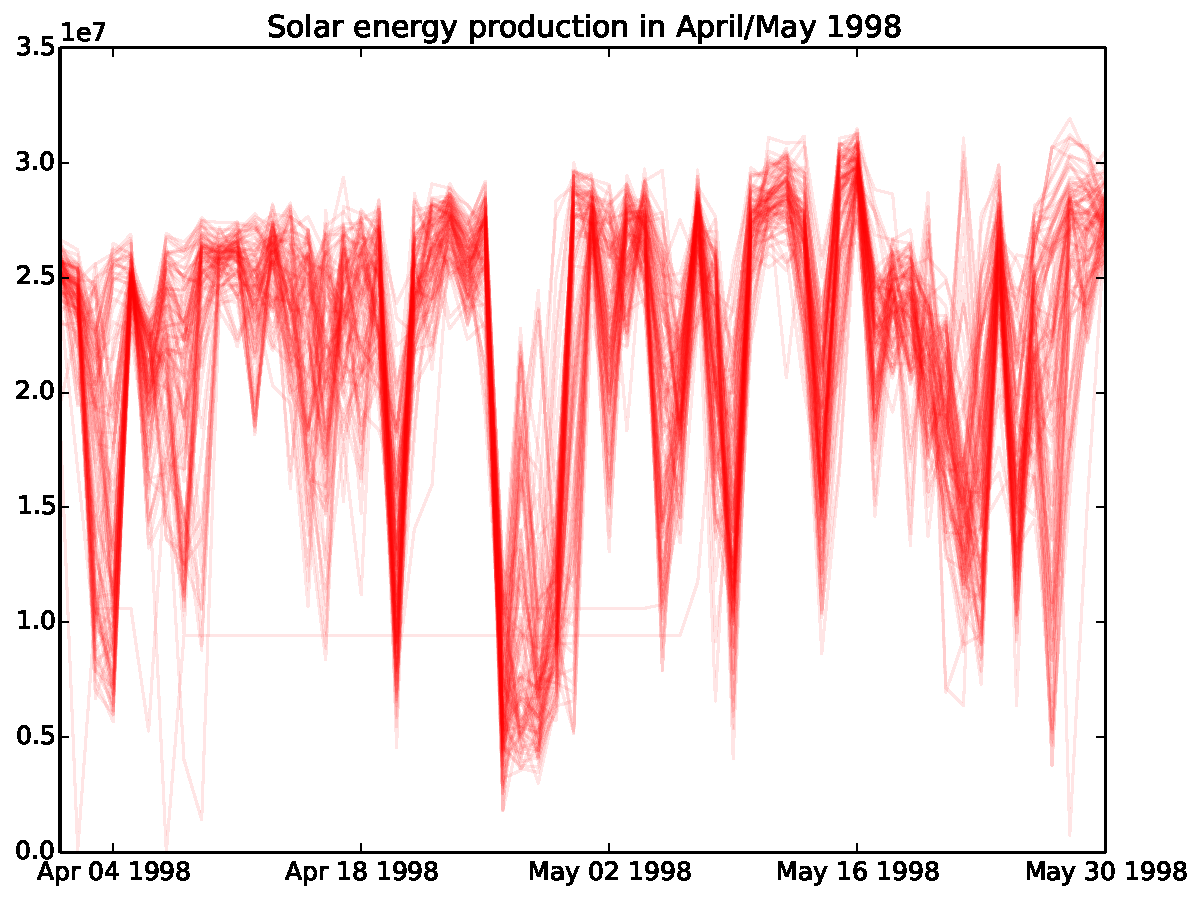
\includegraphics[width=\textwidth]{images/volatility.pdf}
  \end{figure}

\end{column}
\end{columns}
\end{frame}


% Slide 2 =====================================================================

\begin{frame}{Data}

\begin{columns}[T]
    \begin{column}{.45\textwidth}

\begin{block}{Solar energy production}
  \begin{itemize}
     \item 98 Oklahoma Mesonet sites
     \item Total incoming solar energy in $J m^{-2}$
     \item Time period: 1994 - 2007
  \end{itemize}
\end{block}

    \end{column}
    \begin{column}{.45\textwidth}

  \begin{figure}
    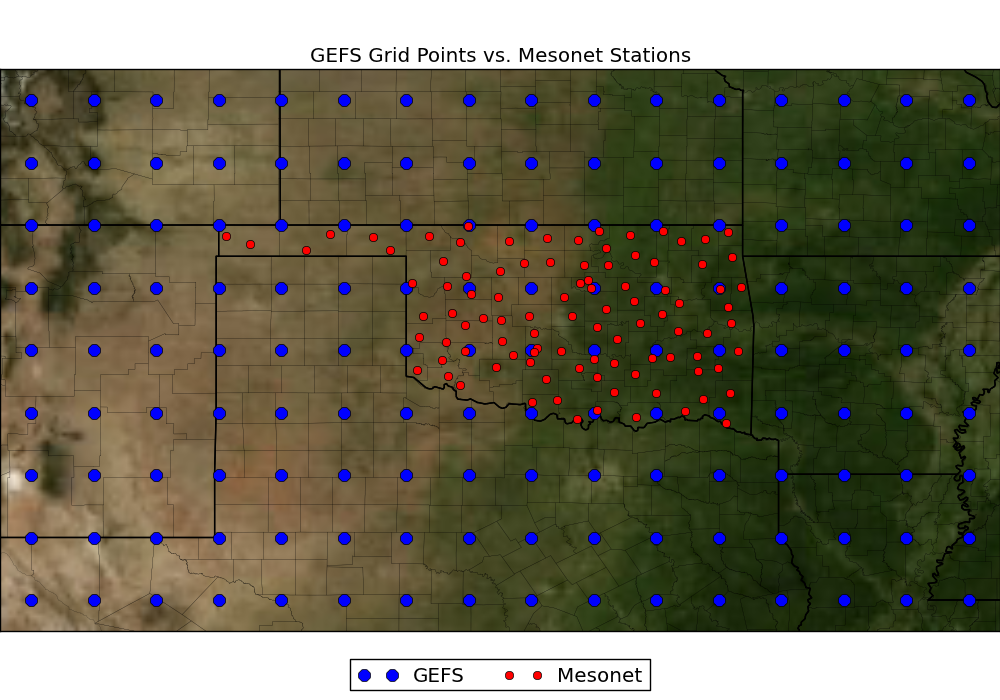
\includegraphics[width=\textwidth]{images/gefs_mesonet_stations.png}\\
    {\color{gray}\tiny{Courtesy: Dr. Amy McGovern}}
  \end{figure}

    \end{column}
  \end{columns}

\begin{block}{Numerical weather prediction}
\begin{itemize}
     \item NOAA/NCEP GEFS Reforecast, 5 forecasts per day
     \item Ensemble comprises 11 members (one control)
     \item 15 variables (temp, humidity, upward radiative flux, ...)
  \end{itemize}
\end{block}

\end{frame}


% Slide 3 =====================================================================

\begin{frame}{Overview of our approach}

\begin{enumerate}
\item Interpolation of meteorological measurements from GEFS grid points onto Mesonet stations;
\item Construction of new features from the interpolated measurements;
\item Prediction of daily energy production using Gradient Boosted Regression Trees.
\end{enumerate}

\end{frame}


% Slide 4 =====================================================================

\begin{frame}{Kriging}

\textbf{Goal:} Obtain local meteorological measurements at each Mesonet station.

\vskip0.5cm

For each day $d$, period $h$ and type $f$ of meteorological measurement:

\begin{enumerate}

\item Build a training set ${\cal L} = \{ (\mathbf{x}_i = (\text{lat}_i,
\text{lon}_i, \text{elevation}_i), y_i = \overline{f_i} ) \}$,  where
$\overline{f_i}$ is the average value of $f$ at location $i$, day $d$ and period $h$;

\item Learn a Gaussian Process from ${\cal L}$, for predicting measurements of type $f$ from coordinates;

\item Predict the measurements $f$ at Mesonet stations for day $d$ and period $h$ using their coordinates.

\end{enumerate}

\end{frame}


% Slide 5 =====================================================================

\begin{frame}{Feature engineering}

\end{frame}


% Slide 6 =====================================================================

\begin{frame}{Predicting energy production}

\end{frame}


% Slide 7 =====================================================================

\begin{frame}{Results}

\end{frame}



\end{document}
